\documentclass[conference, 11pt]{IEEEtran}
\IEEEoverridecommandlockouts
% The preceding line is only needed to identify funding in the first footnote. If that is unneeded, please comment it out.
\usepackage{cite}
\usepackage{amsmath,amssymb,amsfonts}
\usepackage{algorithmic}
\usepackage{booktabs}
\usepackage{graphicx}
\usepackage{siunitx}
\usepackage{tablefootnote}
\usepackage{textcomp}
\usepackage{xcolor}
\usepackage{hyperref}
\hypersetup{
    colorlinks=true,
    linkcolor=blue,
    }
\def\BibTeX{{\rm B\kern-.05em{\sc i\kern-.025em b}\kern-.08em
    T\kern-.1667em\lower.7ex\hbox{E}\kern-.125emX}}
\begin{document}

\title{Predictive Modeling for Real Estate Valuation\\
{\footnotesize \textsuperscript{}}
}

\author{
    \IEEEauthorblockN{Raj Garimella}
    \IEEEauthorblockA{\textit{ECS 171 Spring 2024} \\
    \textit{919351073}\\
    \textit{rajgarimella@ucdavis.edu}}
    \and
    \IEEEauthorblockN{Keenan Kalra}
    \IEEEauthorblockA{\textit{ECS 171 Spring 2024} \\
    \textit{920601521}\\
    \textit{kekalra@ucdavis.edu}}
    \and
    \IEEEauthorblockN{Kaushik Pendiyala}
    \IEEEauthorblockA{\textit{ECS 171 Spring 2024} \\
    \textit{920985616}\\
    \textit{kpendiyala@ucdavis.edu}}
    \and
    \IEEEauthorblockN{Brien Pike}
     \IEEEauthorblockA{\textit{ECS 171 Spring 2024} \\
    \textit{922092730}\\
    \textit{bdpike@ucdavis.edu}}
    \and
    \IEEEauthorblockN{Bhavana Rajapadmanaban}
     \IEEEauthorblockA{\textit{ECS 171 Spring 2024} \\
    \textit{918820877}\\
    \textit{brajapadmanaban@ucdavis.edu}}
}

\maketitle

\begin{abstract}
This paper explores how machine learning can be used to predict residential property prices more accurately. Real estate valuations have always been a critical aspect of the housing market. Traditional valuation methods have struggled to keep up with the ever-changing real estate market. These past methods of valuation lacked the forecasting ability that is required to keep up with the dynamic nature of real estate markets. Such valuations however, need to be as precise as possible as they influence a range of decisions from investment strategies and market analysis to property financing. By using a complex dataset that includes factors such as crime rate, distances to highways and employment centers, and pupil-teacher ratio, the authors developed a machine learning model to create a more accurate property price prediction. In doing so, the team underscored the significance of machine learning in enhancing traditional valuation approaches. This allows for more informed decision-making in real estate transactions.

The dataset utilized in this study includes features from the Boston Housing Dataset, which is full of demographic and geographic information. Various machine learning algorithms are then utilized and discussed, including linear regression, polynomial regression, random forests, and artificial neural networks, to identify the most effective model for price prediction. By comparing the performance of these models, the advantages and limitations of each approach in capturing the complex relationships inherent in the housing market data is demonstrated.


\end{abstract}

\section{Introduction}
Property valuation has long been a cornerstone of the real estate market, proving especially useful in areas such as investment analysis, estate planning, and financing. Accurate prediction of real estate values enhances decision-making in these domains, often leading to significant financial gains. Traditionally, property valuation methods such as the sales comparison approach, cost approach, and income approach have been used to predict real estate values. However, these approaches are highly subjective and involve a tedious process, raising several ethical and efficiency concerns. The National Association of Realtors (NAR) has highlighted issues such as discrimination, a shortage of appraisers, and subjectivity in the appraisal process, advocating for automated valuation methods as an alternative \cite{b1}.

In the realm of real estate, property valuation is not only essential for individual transactions but also for broader economic planning and policy-making. The accuracy of these valuations has far-reaching implications, influencing market stability and investment strategies. Traditional appraisal methods, while foundational, are increasingly challenged by their inherent subjectivity and the potential for human error. These issues are exacerbated by the growing complexity and size of modern real estate markets, necessitating more reliable and efficient valuation techniques.

Among these automated methods, machine learning algorithms provide an objective and efficient alternative, making them a front runner for real estate valuation. Machine learning's ability to analyze complex relationships in large datasets and deliver accurate predictions helps to address the concerns highlighted by the NAR. This paper focuses on the application of various machine learning techniques to the Boston Housing Dataset, aiming to develop models that deliver precise and unbiased real estate value predictions. The comparative analysis of methods such as linear regression, polynomial regression, random forests, and artificial neural networks provides insights into their relative effectiveness and practical implications for the real estate industry.

One of the earliest machine learning techniques was linear regression, which aimed to predict values from the linear relationship between input and output variables. However, datasets with high dimensionality and non-linear relationships require more complex models, such as neural networks and decision trees. In this study, a range of regression techniques, including polynomial regression, random forests, and artificial neural networks, are employed to help provide the most accurate predictions of real estate values.
The Boston Housing Dataset is particularly useful for this analysis due to its extensive array of attributes and data entries, as well as its credibility. The dataset, a subset of the U.S. Census Service data, pertains to housing in Boston, Massachusetts, and provides useful insights into the relationships between its fourteen housing features, which include factors like the age of houses in the neighborhood, proximity to the Charles River, and the median value of residential properties. These characteristics make it an ideal dataset for predictions using machine learning algorithms.

However, while this dataset is useful for making predictions regarding real estate values, it is important to address the ethical concerns regarding it. One of the attributes of the dataset, ‘B’, represents the proportions of blacks by town. This is a product of prejudice and discrimination in the socioeconomic culture when the dataset was created. The dataset is used strictly to train and evaluate machine learning models against pre-existing data and will not be used outside of this context.

This paper explores various machine learning techniques to build models that accurately predict real estate values. By comparing different models, the authors demonstrate how machine learning can improve traditional property valuation methods. The project's goal is to contribute to the ongoing advancement and refinement of real estate valuation practices.

\section{Literature Review}
House price prediction has always been a topic of interest in both the fields of economics and machine learning. Research in the past has used different methods to address this problem such as traditional statistical models to more advanced machine learning techniques. One of the most popular approaches is the use of regression analysis, which has been very promising and widely used in the context of housing price prediction. For instance, Truong et al utilized multiple linear regression to model the relationship between housing prices and predictor variables such as square footage, construction time, and neighborhood characteristics \cite{b2}. However, while regression models have demonstrated reasonable forecast performance, they fail to capture the complex nonlinear relationships that are inherent in real estate markets. To address this, recent studies have focused on machine learning algorithms such as random forests and gradient boosting machines. In one instance, Ho et. al employed a GBM model to predict housing prices in urban areas which achieved higher accuracy compared to traditional regression techniques \cite{b3}. Additionally, deep learning techniques such as convolutional neural networks and recurrent neural networks have also captured newer, unseen patterns in housing data. Despite these advancements, there are many challenges that remain in accurately predicting housing prices, especially in the world of real estate markets. Additionally, going forward ethical considerations such as potential biases in the data that are related to socioeconomic and ethic disparities need to be carefully addressed in future research. 

\section{Dataset Description}

\subsection{Overview}
For this project the authors used a real estate dataset from Kaggle to model home prices from the Boston suburbs using supervised learning techniques. This dataset contains a feature set that has been proven to potentially influence the price of residential properties. It centers around housing in the suburbs of Boston and encompasses 506 instances with 13 continuous attributes alongside one binary-valued attribute. The attributes include per capita crime rate by town (CRIM), proportion of residential land zoned for large lots (ZN), proportion of non-retail business acres per town (INDUS), a dummy variable indicating adjacency to the Charles River (CHAS), nitric oxides concentration (NOX), average number of rooms per dwelling (RM), proportion of owner-occupied units built before 1940 (AGE), weighted distances to Boston employment centers (DIS), an index of accessibility to radial highways (RAD), full-value property-tax rate per \$10,000 (TAX), pupil-teacher ratio by town (PTRATIO), a calculated value based on the proportion of Blacks in the area (B), and the percentage of the lower status of the population (LSTAT). The binary attribute provides information on the proximity of a tract to the Charles River.

\subsection{Exploratory Data Analysis}

To begin the exploratory data analysis (EDA) histograms of the dataset features were plotted ($Fig.
~\ref{fig:histograms}$). Several of the histograms showed skewness and possible outliers, alerting the need to explore normalization and outlier detection. Boxplots of the features were also generated, and they provided a better visual example of the potential outliers in the dataset ($Fig.~\ref{fig:boxplots}$). Finally a correlation heatmap was generated to give an idea of what sort of multicollinearity problems would need to be dealt with ($Fig.~\ref{fig:corr}$).

\begin{figure}
    \centering
    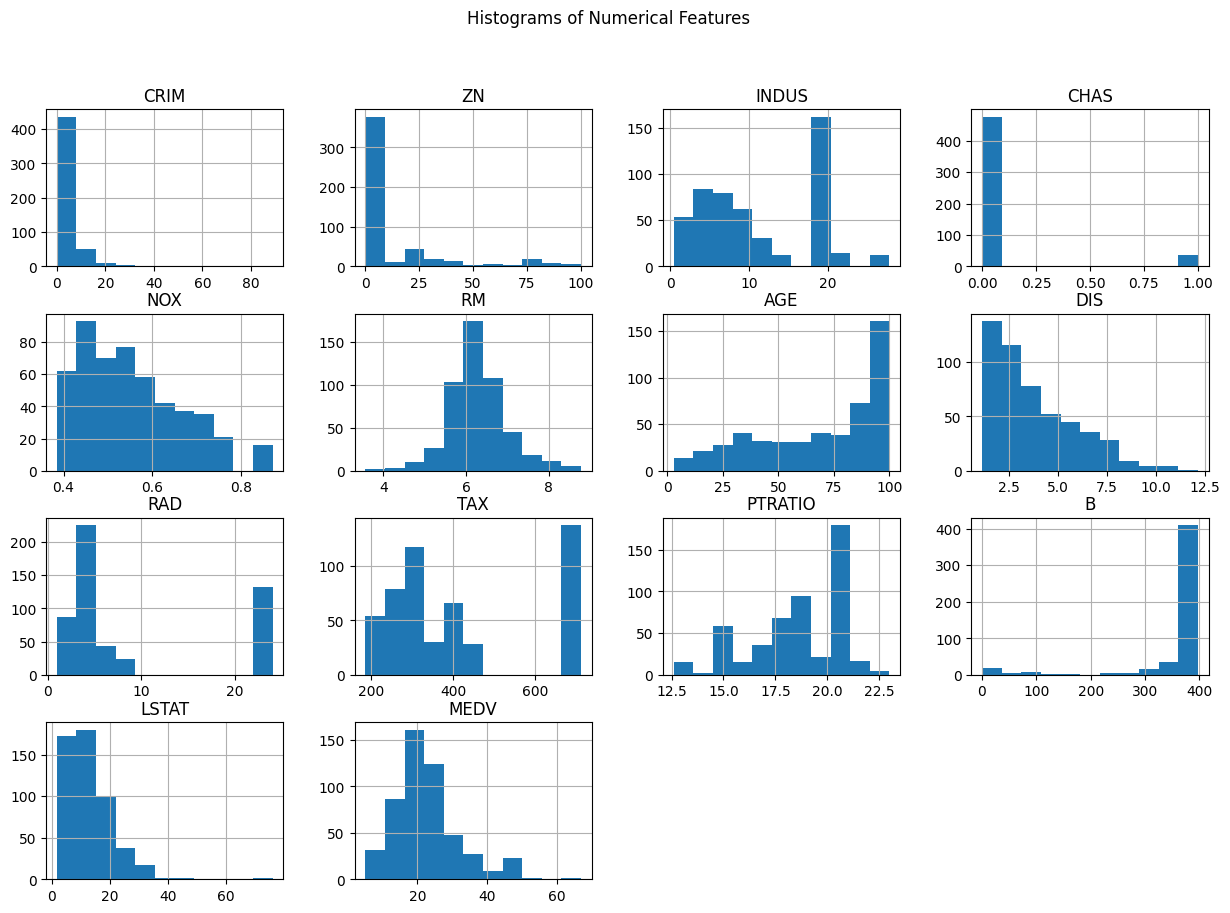
\includegraphics[width=1\linewidth]{histograms.png}
    \caption{Distribution of Features}
    \label{fig:histograms}
\end{figure}

\begin{figure}
    \centering
    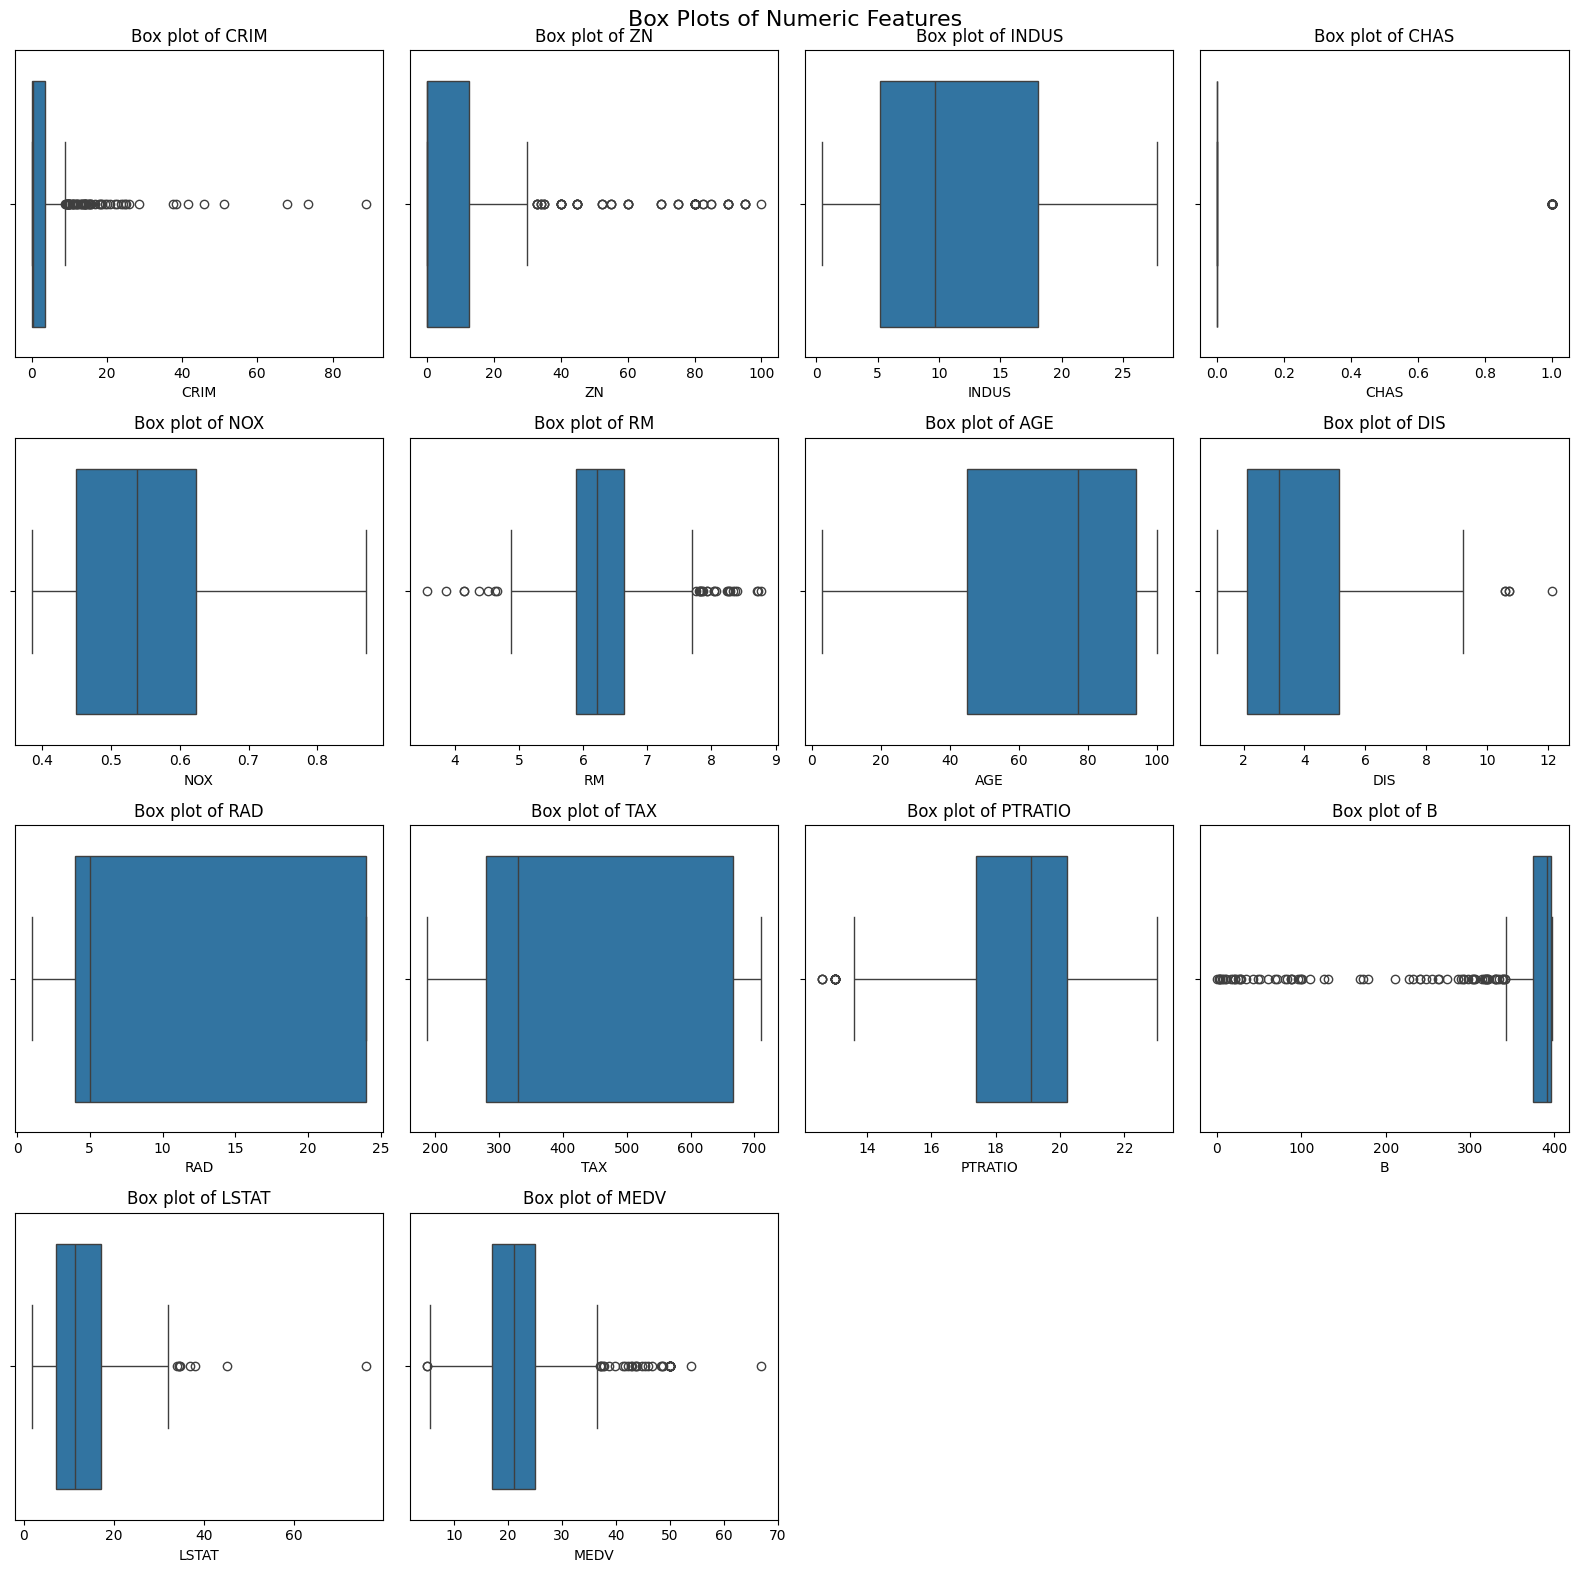
\includegraphics[width=1\linewidth]{boxplots.png}
    \caption{Boxplots of Features}
    \label{fig:boxplots}
\end{figure}

\begin{figure}
    \centering
    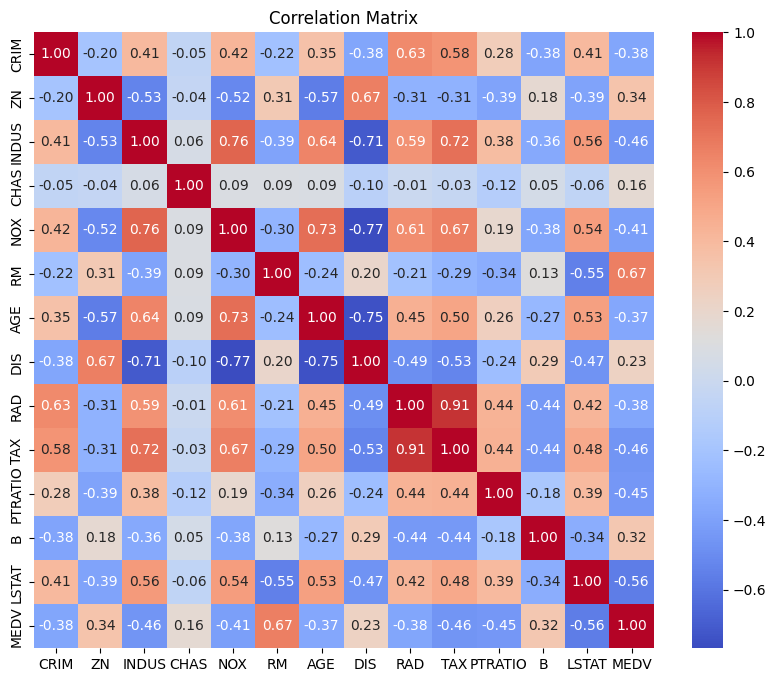
\includegraphics[width=1\linewidth]{heatmap.png}
    \caption{Correlation Heat Map}
    \label{fig:corr}
\end{figure}

Fortunately, the dataset had only five missing datapoints (all were removed prior to further processing) which ensured the project a comprehensive and reliable foundation for analysis and modeling. Initially, the dataset comprised thirteen features pertinent to real estate pricing. However, during the preprocessing phase, the team encountered challenges such as multicollinearity and observed skewed distributions in certain features which were visually seen by box plots. To mitigate these issues, a comprehensive exploratory data analysis was conducted, followed by Z-score normalization, and then outlier detection and removal. Subsequently, a VIF analysis was employed to spotlight and retain the most influential features. This process led to the refinement of our dataset to seven features. This action eased multicollinearity concerns and enhanced future model performance. At the end of EDA a simple polynomial model of the 1$^{st}$ degree was modeled and plotted to provide a baseline metric for model performance ($Fig.~\ref{fig:linear}$).

\begin{figure}
    \centering
    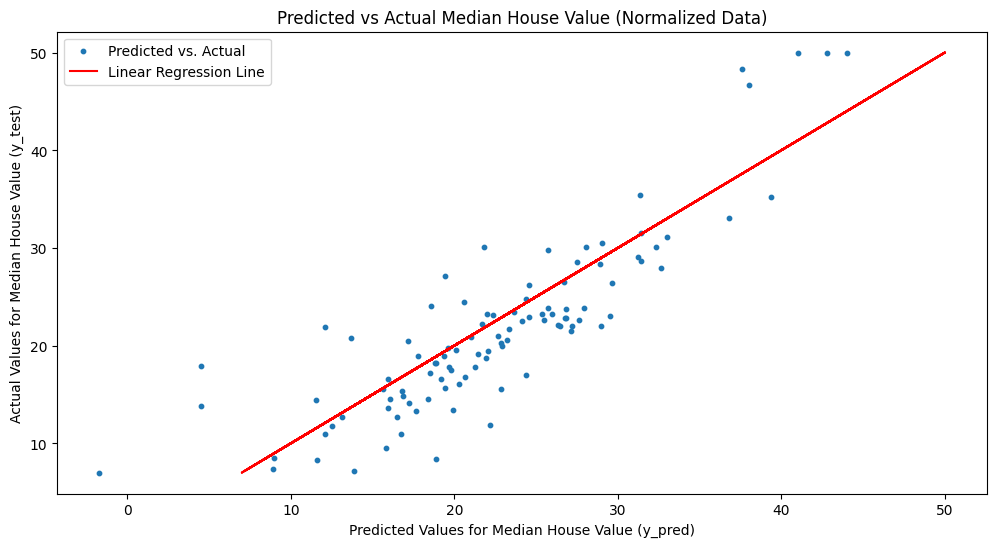
\includegraphics[width=1\linewidth]{linear.png}
    \caption{Linear Model}
    \label{fig:linear}
\end{figure}

\section{Methodology}

\subsection{Feature Selection}

Prior to model selection, the first order of business was feature selection. Feature selection is an important step in the machine learning process for a number of reasons. First, feature selection helps to reduce over-fitting the model by removing features that are redundant or irrelevant to optimal performance. Feature selection also helps to improve the interpretation of the final model by simplifying the feature set to only what is the most important. Finally the accuracy of the model is improved when the authorsare able to focus on the features that contribute most to the model performance. 

For the first step in the feature selection process, correlation between the variables was investigated. A Correlation heat map indicated strong correlation between several variables and TAX. The first attempt at feature selection was done after outlier removal using one-class support vector machine algorithms (SVM). This led to an unexpected result where the variance inflation factors (VIF) became highly inflated, and removal of features, until all VIF values were under our nominal acceptable value of eight, led to removal of six features and severe under-fitting of the model ($Table~\ref{table:vif1}$). 

\begin{table}[htbp]
  \centering
  \caption{vif post outlier removal}
    \begin{tabular}{rrrrr}
    \multicolumn{1}{l}{Feature} & \multicolumn{1}{l}{VIF} &       & \multicolumn{1}{l}{Feature} & \multicolumn{1}{l}{VIF} \\
    \cmidrule{1-2}\cmidrule{4-5}
    \multicolumn{1}{l}{CRIM} & 2.115851 &       & \multicolumn{1}{l}{CRIM} & 2.067497 \\
    \multicolumn{1}{l}{ZN} & 2.761664 &       & \multicolumn{1}{l}{ZN} & 2.236767 \\
    \multicolumn{1}{l}{INDUS} & 14.34520 &       & \multicolumn{1}{l}{INDUS} & 6.593864 \\
    \multicolumn{1}{l}{CHAS} & 1.159081 &       & \multicolumn{1}{l}{CHAS} & 1.090327 \\
    \multicolumn{1}{l}{NOX} & 72.83365 &       & \multicolumn{1}{l}{DIS} & 3.794983 \\
    \multicolumn{1}{l}{RM} & 71.79133 &       & \multicolumn{1}{l}{RAD} & 4.641539 \\
    \multicolumn{1}{l}{AGE} & 19.27237 &       & \multicolumn{1}{l}{LSTAT} & 5.345903 \\
    \multicolumn{1}{l}{DIS} & 13.99453 &       &       &  \\
    \multicolumn{1}{l}{RAD} & 15.05328 &       &       &  \\
    \multicolumn{1}{l}{TAX} & 60.34101 &       &       &  \\
    \multicolumn{1}{l}{PTRATIO} & 84.29239 &       &       &  \\
    \multicolumn{1}{l}{B} & 19.91525 &       &       &  \\
    \multicolumn{1}{l}{LSTAT} & 7.892532 &       &       &  \\
          &       &       &       &  \\
    \multicolumn{4}{l}{$^{\mathrm{a}}$Right side shows VIF post feature removal.}
    \end{tabular}%
  \label{table:vif1}%
\end{table}%

Next the authors tried feature selection prior to outlier removal and got much more predictable results. TAX was found to have the highest VIF score and removal of this lone feature brought all values down under five. This left a total of twelve features in the model and fixed the under-fitting issue.

\begin{table}[htbp]
  \centering
  \caption{vif pre outlier removal}
    \begin{tabular}{lrrrr}
    Feature & \multicolumn{1}{l}{VIF} &       & \multicolumn{1}{l}{Feature} & \multicolumn{1}{l}{VIF} \\
\cmidrule{1-2}\cmidrule{4-5}    CRIM  & 1.778292 &       & \multicolumn{1}{l}{CRIM} & 1.777991 \\
    ZN    & 2.304563 &       & \multicolumn{1}{l}{ZN} & 2.192431 \\
    INDUS & 3.984216 &       & \multicolumn{1}{l}{INDUS} & 3.223914 \\
    CHAS  & 1.073287 &       & \multicolumn{1}{l}{CHAS} & 1.057648 \\
    NOX   & 4.379923 &       & \multicolumn{1}{l}{NOX} & 4.353507 \\
    RM    & 2.839676 &       & \multicolumn{1}{l}{RM} & 1.648364 \\
    AGE   & 3.999108 &       & \multicolumn{1}{l}{AGE} & 2.837585 \\
    DIS   & 7.434675 &       & \multicolumn{1}{l}{DIS} & 3.996417 \\
    RAD   & 9.032710 &       & \multicolumn{1}{l}{RAD} & 2.743238 \\
    TAX   & 1.768444 &       & \multicolumn{1}{l}{PTRATIO} & 1.757768 \\
    PTRATIO & 1.341237 &       & \multicolumn{1}{l}{B} & 1.340387 \\
    B & 2.204576 &       & \multicolumn{1}{l}{LSTAT} & 2.204370 \\
    LSTAT & 2.204576 &       &       &  \\
          &       &       &       &  \\
    \multicolumn{4}{l}{$^{\mathrm{a}}$Right side shows VIF post feature removal.}
    \end{tabular}%
  \label{table:vif2}%
\end{table}%

\subsection{Model Selection}

After feature selection was complete it was time to employ various machine learning algorithms to find the most appropriate fit for the model. Given that this data is structured and highly suited to regression the primary machine learning algorithms the authors used for this analysis were k-fold cross-validation (k-fold), artificial neural networks (ANN), and the ensemble learning technique, random forest.
The first machine learning algorithm employed on this data was k-fold. K-fold cross-validation employing polynomial regression works by partitioning the data in k folds with each fold containing ~ 1/k of the dataset (i.e., ten folds would each contain one-tenth of the data). Then k iterations are performed, each time using $k – 1$ folds for training and the remaining fold for validation. In the first iteration, fold 1 is the validation set, and folds two through k are the training set. In the second iteration fold two becomes the validation set, etc. By partitioning the data in this manner and training the model this way it ensures that every data point appears in the validation set exactly one time. For every iteration, the model is trained on the training dataset and its performance is evaluated on the test dataset. The MSE is recorded for each fold and then this process is iterated over for every polynomial degree tested. The MSE from each polynomial model for each k fold is compared and the best model is chosen ($Figure~\ref{fig:kfold1}$).

\begin{figure}
    \centering
    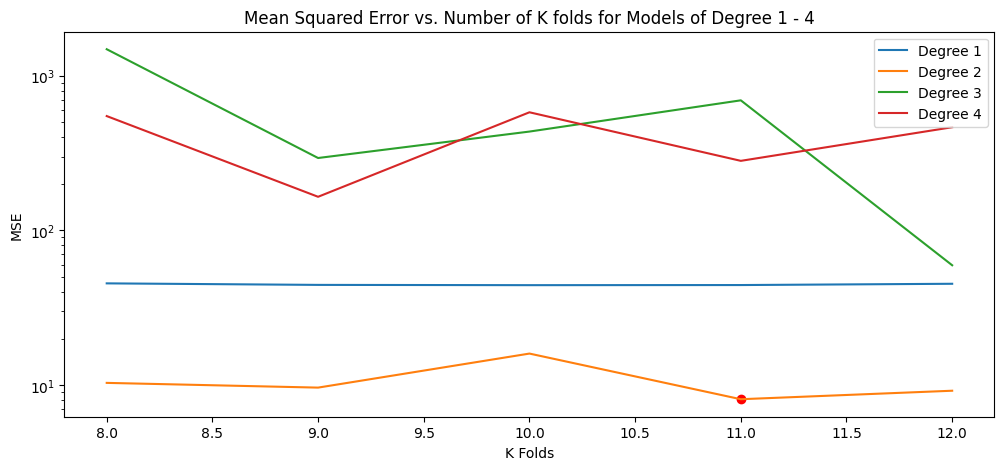
\includegraphics[width=1\linewidth]{K-fold plot.png}
    \caption{K-fold Cross Validation}
    \floatfoot{\footnotesize Logarithmic scale used on Y axis to better visualize MSE between model types.}
    \label{fig:kfold1}
\end{figure}

The next machine learning algorithm attempted was random forest. Random forest is an ensemble learning technique well suited to regression tasks in machine learning. It operates by constructing a forest of decision trees during training and outputting the average prediction of the individual trees to improve predictive accuracy and control for over-fitting. This method leverages the principle of bootstrapping, where each decision tree is trained on a different subset of the training data (sampled with replacement). By averaging the results of these trees, the random forest regressor reduces the variance that can occur with individual decision trees, resulting in more robust and generalizable models. Random forest also incorporates random feature selection, where at each split in the decision tree, a random subset of features is considered, rather than evaluating all features. This adds diversity among the trees, further improving the overall performance of the ensemble. This approach is particularly efficient in handling higher dimensionality or large datasets with many features. For hyperparameter tuning of the random forest regressor the number of estimators was modeled from 10 to 200 in increments of 10 and the model with the lowest MSE was chosen ($Figure~\ref{fig:randomforest}$).

\begin{figure}
    \centering
    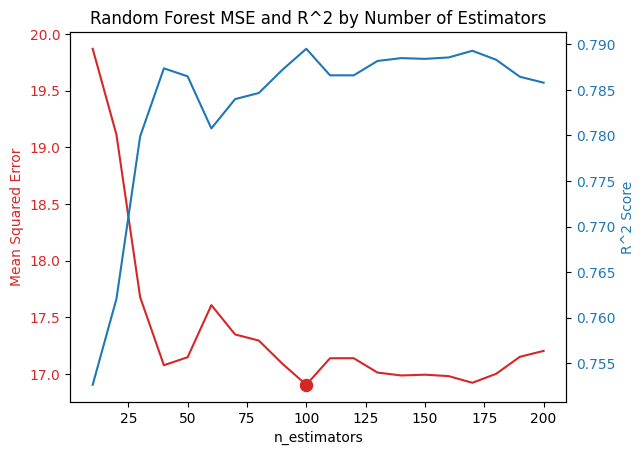
\includegraphics[width=1\linewidth]{Random Forest.png}
    \caption{Random Forest Regressor}
    \label{fig:randomforest}
\end{figure}

The third algorithm employed was artificial neural networks (ANN). ANNs are computational models inspired by the human brain's neural architecture, consisting of interconnected layers of nodes or neurons. These layers include the input layer, hidden layers, and the output layer. The input layer receives external data, which is then processed through one or more hidden layers using weighted connections. Each neuron applies a mathematical function, typically a nonlinear activation function, to the input it receives and passes the result to the subsequent layer. This structure allows ANN’s to model complex patterns and relationships in data, making them highly suitable for regression tasks.
The power of ANNs lies in their ability to learn from data through training. During training, the network adjusts the weights of the connections based on the error of its predictions compared to the actual outcomes. This is achieved using algorithms such as backpropagation, which propagates the error backward through the network and updates the weights to minimize it. Through multiple iterations and with enough data, ANN’s can learn to approximate highly complex functions and make accurate predictions. For this analysis, gridsearch was used to find the optimal set of hyperparameters for: batch size, epochs, activation function, dropout rate, number of hidden layers and neurons per layer. The optimal set of hyperparameters was chosen and MSE was plotted against number of epochs ($Figure~\ref{fig:ANN}$).

\begin{figure}[h!]
    \centering
    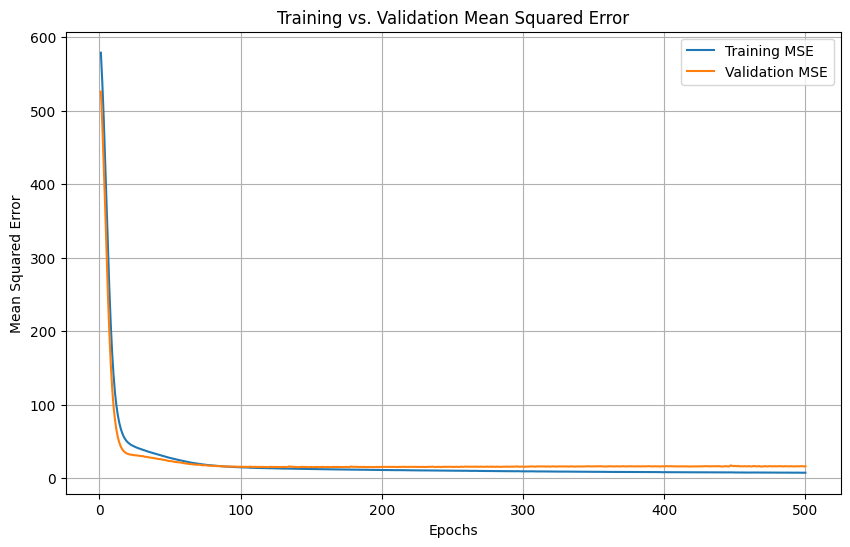
\includegraphics[width=1\linewidth]{ANN.png}
    \caption{Artificial Neural Network}
    \label{fig:ANN}
\end{figure}
\section{Results}
Our primary metric to evaluate and compare models was mean squared error (MSE).
\[
MSE = \frac{1}{n}\sum_{i=1}^n(y_i - \hat{y_i})^2
\]
where $y_i$ is the $i^{th}$ observation and $\hat{y_i}$ is the $i^{th}$ prediction. It measures the ability of the model to effectively predict the overall dataset. However, the units of MSE are the square of the target variable, in this case, dollars squared. This makes interpretation difficult.

To mitigate this, the authors also used root mean squared error (RMSE) for the sake of interpretation.
\[
RMSE = \sqrt{MSE}
\]
RMSE has the same units as the target variable: dollars. It represents the average magnitude of the error of a prediction.

The authors also used $R^2$. $R^2$ ranges from 0 to 1 and represents the proportion of the variance that can be explained by the dependant variables using the model.
\[
R^2 = 1 - \frac{SS_{RES}}{SS_{TOT}} = \frac{\sum_{i=1}^n(y_i - \hat{y_i})^2}{\sum_{i=1}^n(y_i - \bar{y})^2}
\]
However, note that overfitting can lead to higher $R^2$ even if predictive ability does not improve. Thus, the authors used $R^2$ only as a supplementary metric rather than 
 an evaluation criteria.
the authors performed K-fold validation on our polynomial regression model. The authors tested all possible combinations of polynomial degrees 1-4 and fold counts 8-12 ($Table~\ref{tab:kfolds2}$). In addition to recording the MSE, the authors also recorded the total error. 

\begin{table}[htbp]
  \centering
  \caption{K-folds MSE and R$^2$ by Polynomial Degree}
    \begin{tabular}{cccc}
    \toprule
   Degree & K-folds & MSE & R2 \\
    \midrule
    1     & 5     & 43.27308 & 0.556015 \\
    1     & 6     & 44.05266 & 0.528629 \\
    1     & 7     & 43.18468 & 0.535147 \\
    1     & 8     & 43.26791 & 0.54167 \\
    1     & 9     & 43.20002 & 0.530279 \\
    1     & 10    & 43.28442 & 0.565221 \\
    1     & 11    & 42.43232 & 0.555494 \\
    1     & 12    & 43.44481 & 0.567593 \\
    \hline
    2     & 5     & 44.9205 & 0.538384 \\
    2     & 6     & 37.84894 & 0.563027 \\
    2     & 7     & 27.96206 & 0.688607 \\
    2     & 8     & 31.32741 & 0.648528 \\
    2     & 9     & 28.88776 & 0.662653 \\
    2     & 10    & 28.18027 & 0.696613 \\
    2     & 11    & 27.38973 & 0.700704 \\
    2     & 12    & 27.63944 & 0.693835 \\
    \hline
    3     & 5     & 882578 & -9699.12 \\
    3     & 6     & 56609.48 & -662.888 \\
    3     & 7     & 6634.118 & -73.9815 \\
    3     & 8     & 6464.594 & -66.8616 \\
    3     & 9     & 3132.896 & -34.1756 \\
    3     & 10    & 2942.275 & -29.914 \\
    3     & 11    & 3110.491 & -31.3294 \\
    3     & 12    & 1971.134 & -21.7538 \\
    \hline
    4     & 5     & 1344374 & -14125.5 \\
    4     & 6     & 399437.8 & -4750.67 \\
    4     & 7     & 431323 & -4553.69 \\
    4     & 8     & 197453.2 & -1732.57 \\
    4     & 9     & 449794.3 & -6013.28 \\
    4     & 10    & 1446182 & -15644.5 \\
    4     & 11    & 361858 & -3916.09 \\
    4     & 12    & 405152.4 & -4327.1 \\
    \bottomrule
    \end{tabular}%
  \label{tab:kfolds2}%
\end{table}%


The authors used total error to estimate whether or not the a model was a good fit.
\[
\text{Total Error} = \text{Bias}^2 + \text{Variance} + \text{Irreducible Error}
\]
\[
\text{Bias}^2 = E[E[g(x)] - f(x))^2]
\]
\[
\text{Variance} = E[E[g(x)] - g(x))^2]
\]
where g(x) is the model, $E[g(x)]$ is the average prediction and f(x) is the ground truth.
The authors recorded the total error and MSE of each combination of folds and degrees.

$\text{Bias}^2$ represents the error between the model's average prediction and the ground truth while Variance represents the error between the model's average prediction and prediction. High $\text{bias}^2$ and low variance indicates underfitting while low $\text{bias}^2$ and high variance indicates overfitting. Both being low indicates the model is a good fit. The irreducible error depends on the data, not the model, so the authors ignored it and used a modified formula for total error.
\[\text{Total Error} = \text{Bias}^2 + \text{Variance} \]
A good low total error indicates that the model is a good fit while a high total error indicates a bad fit (either over or underfitting).

The best model using polynomial regression and k-fold validation had a degree of 2 (quadratic) and 11 folds. It had an MSE of 27.38973 and an adjusted R$^2$ of 70.10704\%. Although it did not have the lowest total error, it still had a relatively low total error which indicates that the model was a good fit.

Next the authors used random forest and recorded the MSE for the different number of estimators that they tried ($Table~\ref{tab:rf_estimators_mse}$).

\begin{table}[h!]
    \centering
    \caption{Random Forest MSE with Different Number of Estimators}
    \begin{tabular}{|c|c|c|}
        \hline
        N Estimators & MSE & $\text{R}^2$ \\
        \hline
        50  & 17.118529 & 0.786861\\
        100 & 17.136290 & 0.786639\\
        150 & 17.040504 & 0.787832\\
        200 & 17.27837 & 0.784870\\
        \hline
    \end{tabular}
    \label{tab:rf_estimators_mse}
\end{table}

The best random forest model had 150 estimators. It had an MSE of 17.040504 and R$^2$ of 0.787832. However, these differences were quite small, as the difference between the best and worst MSE was less than $1.5\%$ and the difference between the highest and lowest R$^2$ was less than 0.5$\%$. All of the random forest models had MSEs slightly above 17. This was a significant improvement from the best polynomial regression. The R$^2$ on the random forest regressor was also a significant improvement.

The authors also used neural networks to predict the housing price. The input layer had a fixed size--it was required to be equal to the number of input features. Similarly, since the authors were predicting a single target variable, the output layer was fixed at one neuron. Furthermore, the housing price the authors were trying to predict could have a wide range of values. Therefore, the authors used the ReLU activation function in the output layer. Other activation functions such as sigmoid or tanh have upper bounds that would make it impossible to accurately predict the price.

Given these restrictions, the authors still had a lot of freedom in how the authors structured the network. The authors varied the dropout rate, number of hidden layers, number of layers per neuron, activation function, epochs, and batch size. The authors performed grid search to find the best combination. The full search grid parameters were tabulated ($Table~\ref{tab:ann search grid}$). 

\begin{table}[h]
\centering
\caption{Hyperparameter Search Grid}
\begin{tabular}{|c|c|c|c|}
\hline
Dropout Rate & 0 & 0.2 & 0.4 \\
\hline
# Hidden Layers & 1 & 2 & 3 \\
\hline
Neurons per Layer & 10 & 20 & 30 \\
\hline
Activation Function & Relu & Tanh & - \\
\hline
Epochs & 100 & 200 & - \\
\hline
Batch Size & 10 & 20 & - \\
\hline
\end{tabular}
\label{tab:ann search grid}
\end{table}

The best model had the following hyperparameters: 
\begin{itemize}
    \item Dropout rate: 0
    \item Hidden layers: 1
    \item Neurons per Layer: 30
    \item Activation function: ReLU
    \item Epochs: 200
    \item Batch Size: 10    
\end{itemize}
The authors retrained the best neural network model for 500 epochs ($Fig.~\ref{fig:ANN}$). This resulted in an MSE of 15.914241 and an $R^2$ of 0.801855. The MSE for the neural network was lower than that of either the polynomial regression model or the random forest. Similarly, the R$^2$ was higher than either of the aforementioned models.

Comparing the techniques, the authors see a clear pattern: the more complicated models perform better.

\begin{table}[h!]
\caption{Model Performance Comparison}
\centering
\begin{tabular}{| c | c | c | c |}
  \hline
  & MSE & RMSE & R$^2$ \\
  \hline
  Polynomial Regression & 27.38973  & 5.233520 & 0.700704 \\
  \hline
  Random Forest & 17.040504 & 4.128015 & 0.787832 \\
  \hline
  ANN & 15.914241 & 3.989266 & 0.801855 \\
  \hline
\end{tabular}
\label{table:comparison}
\end{table}

The random forest model offered a $37.8\%$ improvement in MSE  and a $11.1\%$ improvement in R$^2$ relative to the the polynomial regression model. The ANN offered a $6.6\%$ improvement in MSE and a $1.7\%$ improvement in R$^2$ relative to the random forest.

Based on our results the authors expect that an estimation produced by the polynomial regression model will be off by $\$5.23350$ thousand. Similarly, on average the estimation produced by the random forest model will be off by $\$4.128015$ thousand and an estimation produced by the neural network will be off by an average of $\$3.989266$ thousand.

\section{Discussion}
In this study, the authors explored various machine learning techniques for predicting residential property prices using the Boston Housing Dataset. Our primary objective was to compare the effectiveness of different models, including polynomial regression, random forest, and artificial neural networks (ANN).

The polynomial regression model with a degree of 2 and 11-fold cross-validation demonstrated promising results with a relatively low mean squared error (MSE) of 27.38973. This model effectively captured the non-linear relationships present in the dataset, as indicated by the adjusted R$^2$ of 70.10704\%.

The random forest regression, robust in nature and able to handle high-dimensional data brilliantly, came up with an MSE value of 17.040504 for 150 estimators. Though slightly better than the polynomial regression, models had few noticeable performance differences. Therefore, choosing a model based on dataset characteristics is of utmost importance.

The ANN model outperformed the polynomial regression and random forest models, recording the lowest MSE at 15.914241. The grid search for tuning hyperparameters did allow the optimization of the network structure in such a manner that it became an effective learner with generalization from the training dataset. 

However, the good performance of the ANN was likely due to overfitting. When the authors attempted to deploy it in the web demo, the ANN produced results that were off by two orders of magnitude. The random forest model, on the other hand, produced results with relatively small errors, that were in line with expectations. 

Neural networks tend to overfit much more than decision trees. This underscores the difference between theoretical and practical performance and the requirement to check the results rather than assuming that they are correct.

Nevertheless, our random forest, despite being the second best model by MSE, could still effectively predict the housing price. The difference in RMSE indicates that its estimations will be less than $\$150$ worse than the estimations of the ANN. In the context of housing prices, $\$150$ is quite small.

Now, these results underscore the potential of advanced machine learning techniques in increasing the predictive power of real estate property valuation models. The recent dramatic increase in performance by ANNs highlights an expectation that deep learning models can capture incredibly complex patterns and interactions within data—much more than simple models can.

Despite these promising results, it is important to acknowledge the ethical considerations associated with using datasets that contain potentially biased attributes. The Boston Housing Dataset includes features such as the proportion of Black residents by town, which reflects historical prejudices. Ensuring that our models do not perpetuate these biases is crucial for ethical and fair real estate valuation.

\section{Road Ahead/Future Work}
The results of this study provide a strong foundation for future research in the domain of real estate valuation using machine learning techniques. However, several avenues for further exploration remain that could be implemented in the future.

\subsection{Model Enhancements}
Our future work would focus on advancing other advanced machine learning models like gradient boosting machines (GBM), support vector regression (SVR), and convolutional neural networks (CNNs). Furthermore, integrating ensemble learning techniques, such as stacking, could combine the strengths of multiple models to further improve predictive accuracy.

Additionally, more experimentation with hyperparameters and more comprehensive testing of the neural network could yield a model that still has superior performance--possibly even superior to our current best performance--without overfitting. 

\subsection{Feature Engineering}
The enhancement of the feature engineering process could lead to better model performance. By adding in new features such as economic indicators, interest rates, and geographic information data, the authors could have a more comprehensive understanding of the factors influencing property prices. Feature selection techniques, such as principal component analysis (PCA) and recursive feature elimination (RFE), could also be employed to reduce dimensionality and improve model interpretability.

\subsection{Real-world Applications}
The practical utility of these models can be validated through deployment in real-world settings. In this context, establishing cooperation with real estate agencies and financial institutions can provide valuable insights into the testing performance modalities. The development of user-friendly interfaces and integrations with deployed platforms in real estate will facilitate broader adoption and practical use of this model.

\subsection{Longitudinal Studies and Dynamic Modeling}
Longitudinal studies on the values of properties over time would give more profound insight into the temporal dynamics of real estate markets. The development of dynamic models, which can automatically update their predictions at the availability of new data, may provide further relevance and accuracy to the valuation models.

\section{Project Roadmap}
The github repository can be found at this \href{https://github.com/kklike32/171-Real-Estate}{link} and our demo is \href{https://www.youtube.com/watch?v=x0xYc0DO8yo&feature=youtu.be}{here}. Our project deliverables were broken up into key milestones which the authors worked on throughout the quarter. Our first step was choosing an appropriate dataset to work with, as this would determine the direction for the project. After compiling a list of interesting datasets, the authors settled on the \href{https://www.kaggle.com/code/prasadperera/the-boston-housing-dataset}{Boston Housing Dataset} because of its extensive array of attributes and data entries. 

Our next milestone after dataset selection was exploratory data analysis. After familiarizing ourselves with the data, we visualized trends by plotting histograms, boxplots, and heatmaps. We then performed VIF analysis before outlier removal to filter out non-influential features.

After EDA, we experimented with different models and hyperparameters. We experimented with a lot of models including Linear Regression, Decision Tree Regressor, XGBoost, LightGBM, CatBoost, XGBoost with PCA, XGBoost with Regularization & Early Stopping, GCN, GAT, ResNet and Transformer, Ensemble of Multiple Neural Networks, Ridge Regression, Random Forest Regressor, SVR, and XGBoost Regressor. Finally, we decided to implement polynomial regression, random forest regression, and an artificial neural network with a grid search for optimization as they had the best results. We created each of these models and ran it against test data to determine evaluation metrics.

After analyzing our results, we worked on the final report, which summarized our process and findings. Finally, we created a visual presentation and demo for the project, where all of us walked through the process of building these models and our analysis.
\vspace{0.1in}

Below is a list of contributions to the project by the group members.
\vspace{0.1in}

Raj Garimella 
\begin{itemize}
    \item Neural network implementation
    \item Model evaluation and comparison
    \item Write-up focused on results
    \item Miscellaneous edits to the code base and paper
    \item Presentation recording and editing
\end{itemize}
\vspace{0.1in}

Keenan Kalra 
\begin{itemize}
    \item Exploratory Data Analysis
    \item Model Building and Testing
        \begin{itemize}
            \item Neural Network
            \item K-Folds regression
            \item Random Forest
            \item XGBoost
            \item Resnet and Transformer
        \end{itemize}
    \item Flask Development Coding
    \item Write Up Discussion
    \item Write-Up Road Ahead/Future Work
\end{itemize}
\vspace{0.1in}

Kaushik Pendiyala
\begin{itemize}
    \item Data Preprocessing (Missing Values Removal and Standardization)
    \item Exploratory Data Analysis (Linear Regression)
    \item Introduction Write-Up
    \item Project Roadmap Write-Up
    \item Demo Presentation
\end{itemize}
\vspace{0.1in}

Brien Pike
\begin{itemize}
    \item Feature selection
    \item Outlier removal
    \item K-folds regression coding
    \item Random forest regression coding
    \item Flask web app coding
    \item Methodology write up
    \item Miscellaneous editing and formatting 
\end{itemize}
\vspace{0.1in}

Bhavana Rajapadmanaban
\begin{itemize}
    \item Data Preprocessing
    \item Dataset Visualization
    \item Mid Quarter Progress Report
    \item Abstract
    \item Literature Review
    \item Dataset Description
\end{itemize}
\vspace{0.1in}

\begin{thebibliography}{00}
\bibitem{b1} “Valuation / valuation issues update,” National Association Of Realtors, https://narfocus.com/publication-issue/view/2022-06-14-valuation-valuation-issues-update# (accessed Jun. 8, 2024).
\bibitem{b2} Q. Truong, M. Nguyen, H. Dang, and B. Mei, “Housing price prediction via Improved Machine Learning Techniques,” Science Direct, https://www.sciencedirect.com/science/article/pii/S1877050920316318 (accessed Jun. 8, 2024).
\bibitem{b3} W. K. O. Ho, B.-S. Tang, and S. W. Wong, “Predicting property prices with machine learning algorithms,” Journal of Property Research, vol. 38, no. 1, pp. 48–70, Oct. 2020. doi:10.1080/09599916.2020.1832558
\end{thebibliography}
\vspace{12pt}
\end{document}
